% =========================================================================
\chapter{What is an extreme heat day?}
\label{ch:extreme}
% =========================================================================

\section{Percentiles}
Sort a list of values from smallest to largest. The \textbf{$p$-th percentile} is the value below which $p$\% of them
lie. The 99th percentile is the value that only 1\% of the list exceeds.

\begin{example}[A small example]
Take the daily maximum temperatures of 1{,}000 summer days at one cell, sorted. The 99th percentile is (about) the
990th value: only 10 days, 1\%, were hotter. If that value is 33.4\,$^\circ$C, then 33.4\,$^\circ$C is the threshold.
\end{example}

\section{The threshold $u$}
For every \textbf{cell} $c$ and every \textbf{season} $g$, the threshold $u_{c,g}$ is the 99th percentile of the daily
maximum temperature of that cell in that season, using only the years \textbf{1981--2010}.
\begin{itemize}
  \item $529\text{ cells}\times4\text{ seasons}=\textbf{2{,}116 thresholds}$.
  \item A day is an \textbf{extreme heat day} if its maximum temperature is above the threshold of its cell and season:
        $T^{\max}_{c,t}>u_{c,g(t)}$.
  \item By construction, about 1\% of the days of 1981--2010 are extreme in every cell and season.
\end{itemize}

\begin{figure}[H]
\centering
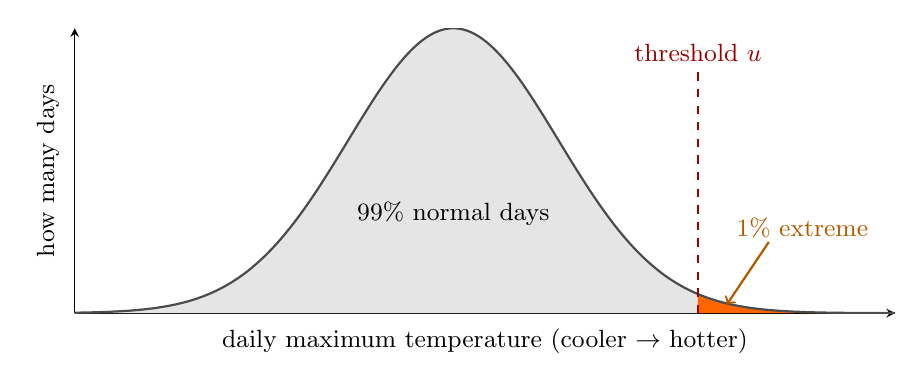
\begin{tikzpicture}
\begin{axis}[width=12cm,height=5.2cm,axis lines=left,xlabel={daily maximum temperature (cooler $\rightarrow$ hotter)},
  ylabel={how many days},xtick=\empty,ytick=\empty,ymin=0,xmin=-3.6,xmax=4.2,samples=200,domain=-3.6:4.2,
  xlabel style={font=\small},ylabel style={font=\small}]
\addplot[fill=black!10,draw=none,domain=-3.6:2.326] {exp(-x^2/2)} \closedcycle;
\addplot[fill=orange!80!red,draw=none,domain=2.326:4.2] {exp(-x^2/2)} \closedcycle;
\addplot[thick,black!70] {exp(-x^2/2)};
\draw[dashed,thick,red!60!black] (axis cs:2.326,0) -- (axis cs:2.326,0.85);
\node[font=\small,red!60!black,anchor=south] at (axis cs:2.326,0.85) {threshold $u$};
\node[font=\small] at (axis cs:0,0.35) {99\% normal days};
\node[font=\small,orange!70!black,anchor=west] at (axis cs:2.6,0.3) {1\% extreme};
\draw[->,orange!70!black,thick] (axis cs:3.0,0.25) -- (axis cs:2.6,0.03);
\end{axis}
\end{tikzpicture}
\caption{All days of one cell and season, from cooler to hotter. Days beyond the threshold (orange) are extreme heat
days. The real shape is not exactly a bell curve; this is only a picture of the idea of a ``tail''.}
\end{figure}

\section{Why a threshold per cell and per season?}
\begin{itemize}
  \item \textbf{Per cell:} 30\,$^\circ$C is a normal summer day in the plains but extreme high up. Each cell is compared
        with its own past. Thresholds fall by 6--7\,$^\circ$C per km of altitude.
  \item \textbf{Per season:} an unusually warm winter day is also an extreme, even though it is cooler than a normal
        summer day.
  \item \textbf{Fixed past (1981--2010):} the thresholds never change, so a warming climate shows up as more extreme days.
\end{itemize}

\section{The label}
The prediction is always about \textbf{tomorrow}. Call today day $D$. The label of a row is
\[
  \text{label}=\begin{cases}1 & \text{if day }D+1\text{ is an extreme heat day in this cell,}\\ 0 & \text{otherwise.}\end{cases}
\]
This is a \textbf{binary classification} problem: the answer is one of two classes, 1 (``extreme'') or 0 (``normal'').

\section{Normal and anomaly}
The \textbf{normal} of a cell for a calendar day is the 1981--2010 average maximum temperature over the 15 days centred
on that date (7 days either side). The \textbf{anomaly} of a day is its temperature minus its normal: $+3$ means 3
degrees warmer than usual for that date.

\section{The climate signal}
With the same fixed thresholds, extreme days were \textbf{1.02\%} of cell-days in 1981--2010 but \textbf{1.94\%} in
2016--2025: almost twice as many. This is also why a model that never warns is 99\% accurate in the old years but only
98\% accurate in the test years.

\begin{sayit}
``A day is extreme if it is hotter than 99\% of that cell's own days in the same season over 1981--2010. That gives
2,116 thresholds, and the task is: will tomorrow be above the threshold here, yes or no?''
\end{sayit}
